This Supplement contains additional information about the data used as well as
details about statistical methodology.

\section{A general description and depiction of convolution}
\label{sec:convol}

In general, the goal of convolution is to propagate the input signal forward in
time using a probability distribution. In the 1D and discrete context, it is
simply a rolling, weighted average of the past. So for an input sequence
$\{x_t\}_{t=1}^n$ and time-constant weights $\{z(k)\}_{k=-\infty}^0$, the output
sequence $\{y_t\}_{t=1}^n$ is given by
\begin{linenomath*}
\begin{equation}
    y_t = \sum_{s=0}^t z(s)x_{t-s}.
\end{equation}
\end{linenomath*}
\Cref{fig:convol} presents a depiction of the convolution procedure for an
example signal $x_t$ (smoothed cases, orange line). Essentially, to push the
cases forward in time, we take the appropriately aligned (forward-in-time) delay
distribution $z(s)$ (blue shaded region) and convolve it with the smoothed cases
signal counts by it to get the convolved  estimates (blue line). This process is
repeated as we march forward in time, as shown through the stop-motion panels,
such that it eventually covers the entire line of cases. An important takeaway
from this is that convolution is not the same as a simple shift of the data.
A shift is a special case: when $z(d)=1$ and $z(s)=0$, $s\neq d$, we shift $x$
forward by $d$. Rather, convolution generally weights the entire past by
non-zero probabilities. Deconvolution proceeds in the same fashion, but in the
opposite direction, going backward in time and undoing the effect of a
convolution. 

\begin{figure}[H]
\centering
    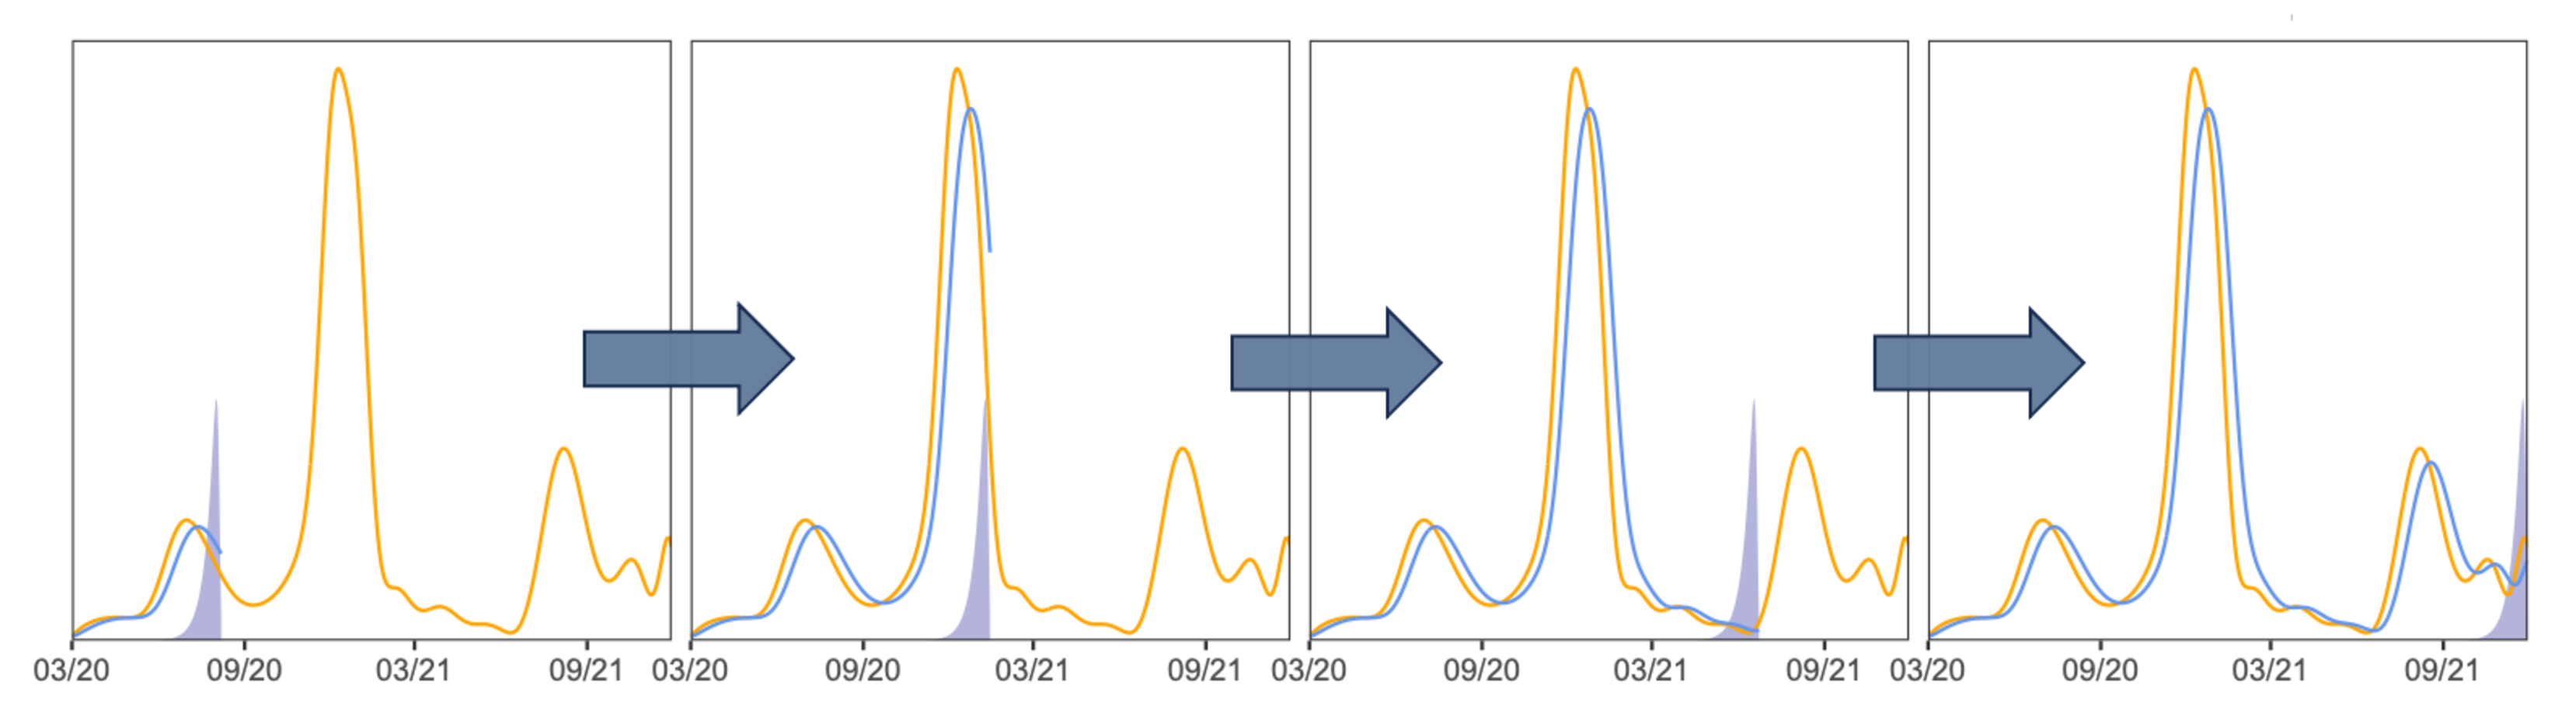
\includegraphics[width=0.99\linewidth]{convolution_diagram.pdf}
    \caption{A general depiction of convolving smoothed cases (orange line) with the corresponding delay probabilities (shaded blue area) to get the convolved estimates (blue line) over four different times.}
    \label{fig:convol}
\end{figure}

\section{Additional details on the date fields in the CDC line list}
\label{sec:linelist-details}

Because the restricted CDC line list is updated monthly and cases may undergo revision, we
use a single version of it that was released on June 6, 2022. We consider this
version to be finalized in that it is well-beyond our study end date such that
the dataset is unlikely to be subject to further significant revisions.

\Cref{tab:order-events-table} presents the percent of pairwise occurrences for
the different possible permutations of events in the line list. Essentially,
most cases follow the idealized ordering shown by
\Cref{fig:chain_events_onset_report} and so we adhere to this construction as
much as possible. Unfortunately, the line list has significant missing data,
notably with respect to our variables of interest. Approximately 62.3\% of cases
are missing the symptom onset date, 55.4\% are missing positive specimen date,
and 8.96\% of cases are missing the report date. Furthermore, cases with missing
report or positive specimen dates may be filled with their symptom onset date
\citep{jahja2022real}. So it is possible that all three variables may have the
same date for a case. However, we only actually deal with pairs of these events;
we do not use all three at once in our construction of the delay distributions.
Therefore, we restrict our investigation of coincident missingness to the possible pairs.
% \Cref{fig:prop-cc} suggests that this issue impacts states differentially due to
% the inconsistent proportions of zero delay between positive specimen and report
% date across states. 

\begin{table}[t!]
    \centering
\begin{tabular}{@{}lp{3cm}p{8.5cm}@{}}
\toprule
\textbf{Order of events}& \textbf{Percent pairwise occurrence} &
\textbf{Handling}\\ \midrule \addlinespace
IO $\rightarrow$ SO $\rightarrow$ PS $\rightarrow$ RE & \begin{tabular}[t]{@{}l@{}}PS $\geq$ SO: 97.1 \\ PS = SO: 33.6\\ PS \textgreater\ RE: 1.74\\  PS = RE: 14.6\end{tabular} & This is the idealized order of events and so the  support sets for  SO $\rightarrow$ PS and PS $\rightarrow$ RE delay distribution constructions around this such that IO comes first by construction, SO typically precedes PS, but may be the same  or come before, and RE comes after PS and SO \\ \addlinespace
IO $\rightarrow$ PS $\rightarrow$ SO $\rightarrow$ RE & \begin{tabular}[t]{@{}l@{}}PS \textless\ SO: 2.91 \\ SO $\leq$ RE: 99.3 \\ SO \textless\ RE: 86.1\end{tabular}            & Allowed for negative delays up to the largest non-outlier value for the 0.05 quantile of delay from PS to SO by state                                                                                                                                         \\ \addlinespace
IO $\rightarrow$ PS $\rightarrow$ RE $\rightarrow$ SO & \begin{tabular}[t]{@{}l@{}}RE \textless\ SO: 0.7 \\ RE \textless\ PS: 1.7\end{tabular}                                    & Current handling by the CDC of the line list ensures that the most concerning cases are handled where SO = PO = RE, SO = RE and PO = RE                                                                                                                                                \\ \addlinespace\bottomrule
\end{tabular}
\caption{Percent pairwise occurrence for the different permutations of events considered in the restricted CDC line list. The abbreviation IO stands for infection onset, SO is symptom onset, PS is positive specimen, and RE is report date. We consider a restricted set of permutations because we assume that IO must come first and that PS must precede report date for a case to be legitimate. Finally, the underlying assumption for the percent pairwise occurrence calculations is that the cases must have both elements present (not missing).}
\label{tab:order-events-table}
\end{table}


Due to the contamination in the zero delay cases (those whose symptom onset was
used to fill missing positive specimen or report date, the true extent of which
is unknown to us), we omit all cases where the positive specimen and report
dates have zero delay from our analysis. We choose to allow for zero and
negative delay for symptom onset to report because correspondence with the CDC
confirms the possibility that a person could test positive before symptom onset
and it is a reasonable ordering to expect if, for example, the individual is
aware that they have been exposed to an infected individual.

\begin{figure}[!tb]
\centering
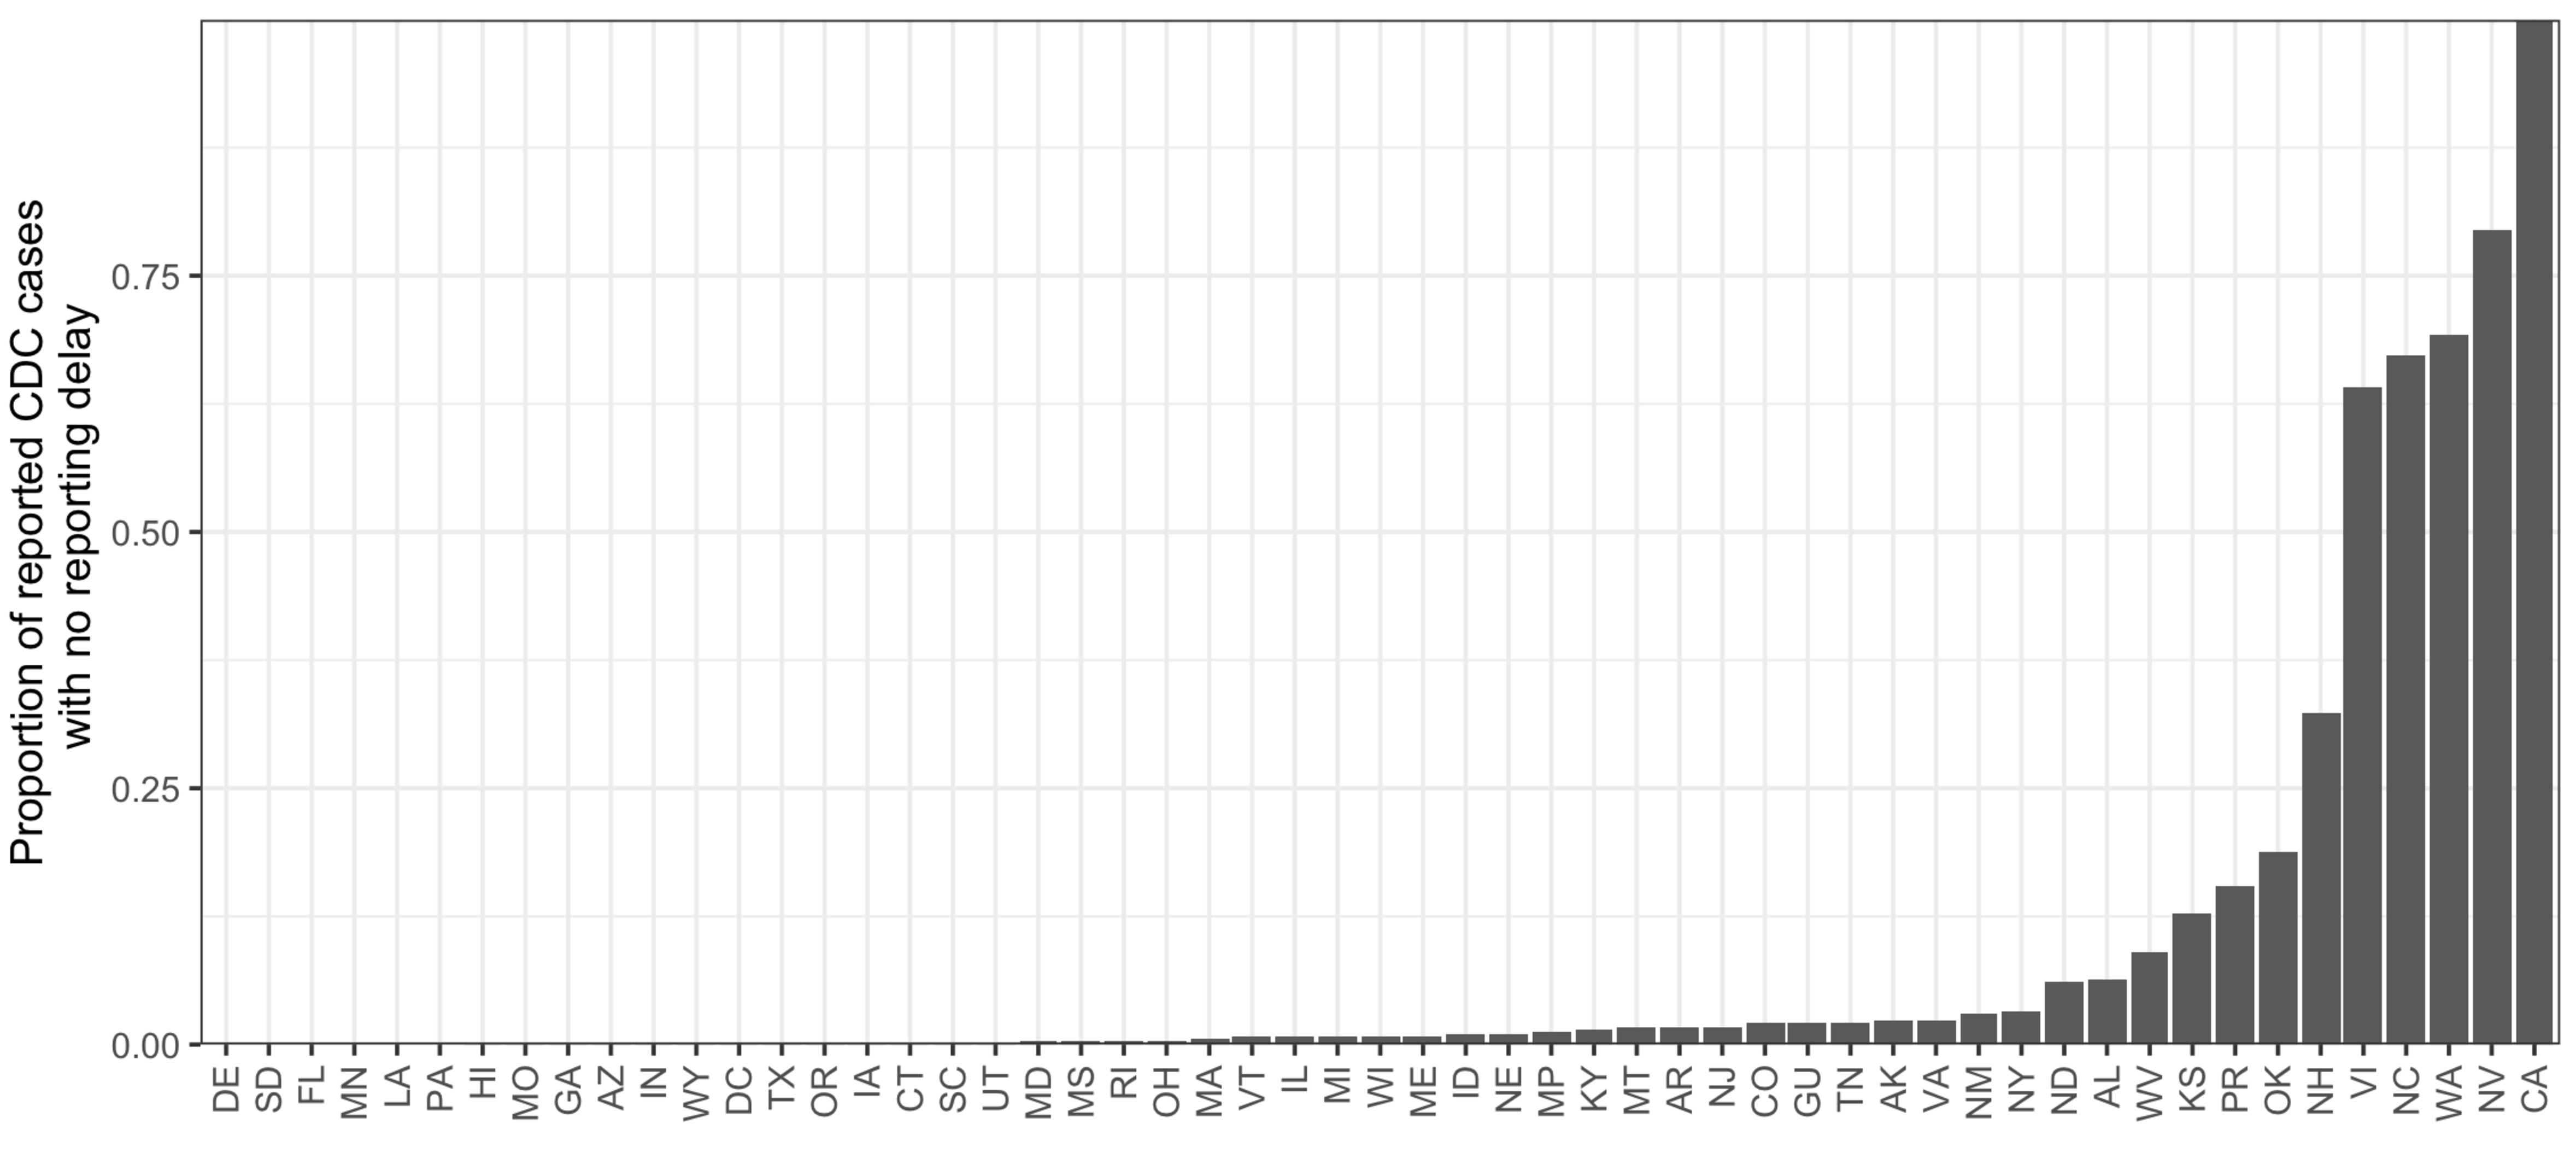
\includegraphics[width=0.9\linewidth]{prop_cc_zero_delay.pdf}\\
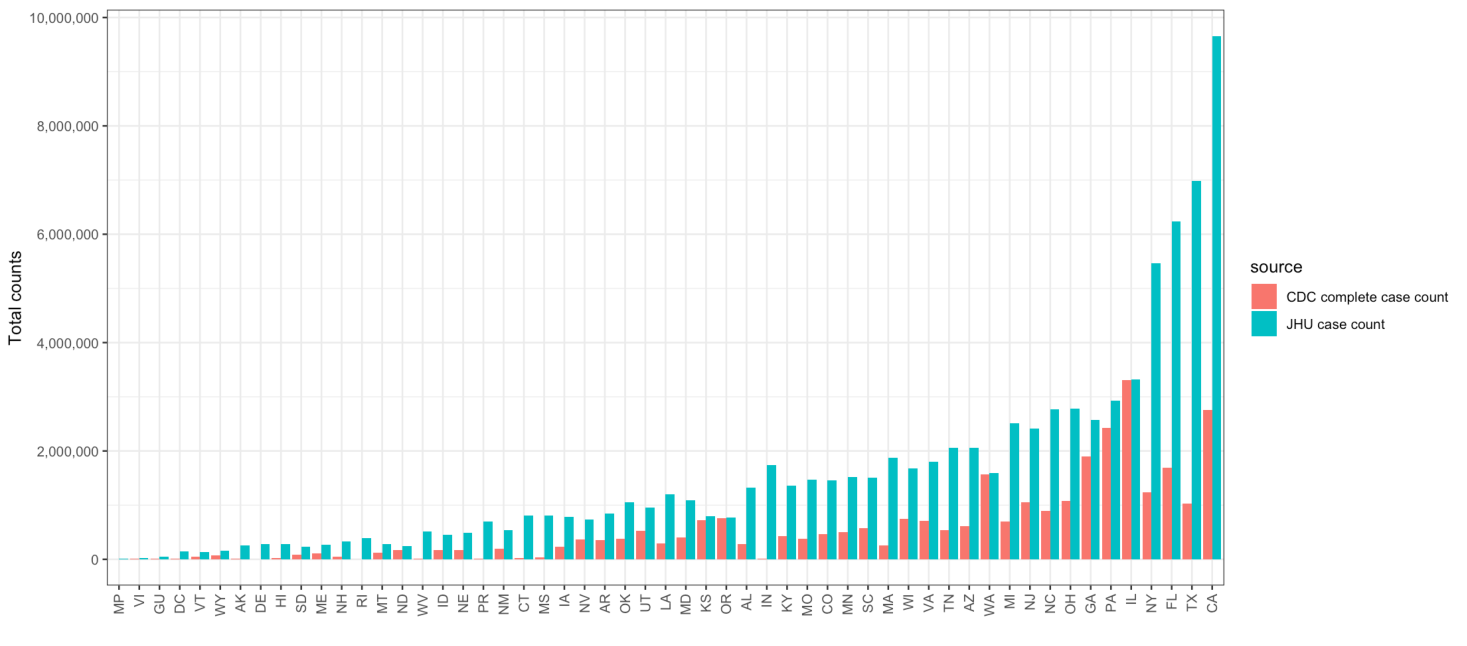
\includegraphics[width=0.9\linewidth]{prop_cc_cdc_vs_jhu.pdf} 
\caption{Top panel: Proportion of complete cases with zero delay between
    positive specimen and report date in the restricted CDC line list dataset.
    Bottom panel: Complete case counts by state in the CDC line list versus the
    cumulative complete case counts from JHU CSSE as of June 6, 2022. All
    counts have been scaled by the 2022 state populations as of July 1, 2022
    from \citep{uscensus2022annual}.}
\label{fig:prop-cc}
\end{figure}

The restricted CDC line list contains 74,849,225 cases (rows) in total compared
to 84,714,805 cases reported by the JHU CSSE; that is, the line list is missing
about 10 million cases. The extent that this issue impacts each state is shown
in \Cref{fig:prop-cc}, from which it is clear the fraction of missing cases is
substantial for many states, often surpassing 50\% \citep{jahja2022real}. In
addition, the probability of being missing does not appear to be the same for
states, so there is likely bias introduced from using the complete case line
list data. We consider such bias to be unavoidable in our analysis due to a lack
of alternative line list sources. 



%\section{Table on the percent pairwise occurrence of events in the CDC line list}


\section{Additional details on delay distribution calculations}
\label{sec:delay-justifications}
\begin{linenomath*}
In the line list, we observe unusual spikes in reporting in 2020 in comparison
to majority of 2021. When stratified by report date, a few states contribute
unusually large case counts on isolated dates very late in the reporting process
(often more than 100 days following specimen collection). These large
accumulations of cases over time are likely due breakdowns of the reporting
pipeline. Such anomalies are not likely to be reliable indicators of the delay
from positive specimen to case report. Therefore, we prune these reporting
backlogs systematically. The heuristic is to find large batches of cases that
were all simultaneously reported on the same date with a lengthy delay (as would
happen if a state ``found'' a tranche of previously unreported positive tests).
For each of three time intervals (delimited by July 16, 2020, 
October 16, 2020, and January 15, 2021), we apply the following pruning procedure:
Let $x_{\ell t}(d)$ be the number of cases in state $\ell$ with positive
specimen collection date $t$ and delay $d$. For each $j=1,2,\ldots$, 
define 
$
z_{\ell bj} = \sum_{d = 50j}^{50(j+1)}\sum_t x_{\ell
t}(d).$ Then, locate the collection of
potentially problematic combinations 
\end{linenomath*}
\begin{linenomath*}
$$
\cH = \{(\ell, b, j) : \log(z_{\ell bj}) >
\textrm{median}_{\ell}(\log(z_{\ell bj})) + 1.5
\times\textrm{IQR}_\ell(\log(z_{\ell bj}))\}.
$$
\end{linenomath*}
Remove any case reports from the line list in $\cH$ where the total number of
cases with the same report date exceeds 2000 if $j=1$ or 500 otherwise.


% For this, we operate only on part of the line list intended for the positive
% specimen to case report delay estimation (as this is where we use case reports
% from the line list). Then, we divide this line list into three roughly
% evenly-spaced and non-overlapping intervals over 2020 and early 2021 (the
% interval end points on July 16, 2020, October 16, 2020, and January 15, 2021).
% For each interval, we separate the cases with reporting delays that are at least
% 50 days long into equally-sized bins of 50 days. Then, for each interval and
% bin, we perform the following pruning procedure:
% \begin{enumerate}[noitemsep]
% \item Obtain the total count of these delays for each state. 
% \item Check whether each such count on the log scale is at
% least the median (for the bin) plus 1.5 times the interquartile range. Retain
% only those that exceed this criterion as candidates for pruning. 
% \item For the candidate states, compute the case counts by report date. 
% \item If there is a report date for a candidate state with a case count greater 
% than or equal to a pre-specified threshold, then remove/prune those cases from the line list. 
% We set the threshold to be 2000 cases for the first two bins, and then lower
% it to 500 for the remaining bins based on inspection.
% \end{enumerate}

Finally, in New Hampshire and for a small handful of report dates, all cases
reported by JHU appear in the CDC line list and all are recorded as having
positive specimen collection date equal to the report date. The resulting
estimate of the delay distribution (see \Cref{sec:step1})
$\widetilde{p}_{\textrm{NH},t}(k)$ would be a point mass at $k=0$ and the weight
$\alpha_{\textrm{NH},t}=1$ resulting $\widehat\pi_{\textrm{NH},t}(k)$ also being a
point mass at $k=0$. In this specific case, we force $\alpha_{\textrm{NH},t} =
\min_{\ell\neq\textrm{NH}} \alpha_{\ell,t}$.

\section{Variant circulation proportions}
\label{sec:variant-proportions}


To estimate the daily proportions of the variants circulating in each state, we
obtain the GISAID genomic sequencing data from CoVariants.org
\citep{hodcroft2021covariants, elbe2017data}. These counts represent the total
number of cases belonging to a particular variant using
a sample of positive tests over a biweekly period. To estimate the population
proportion of each variant, we apply multinomial logistic regression 
for the eight variant categories separately for each state. 
Multinomial logistic regression is a standard technique to model the
frequency of SARS-CoV-2 variants
\citep{obermeyer2022analysis, annavajhala2021emergence, figgins2021sars}.

We let $V_{j\ell,t}$ to be the probability of a new cases at time $t$ in location
$\ell$ corresponding to variant $j$. Let $v_{j\ell,t}$ be the analogous observed
proportion. Then nonparametric multinomial logistic regression models the log odds
as the system
\begin{linenomath*}
\begin{equation}
\log\left(\frac{V_{j\ell,t}}{1-V_{j\ell,t}}\right) = \beta_{j\ell,0} + \beta_{j\ell,1} t + \beta_{j\ell,2}t^2 + \beta_{j\ell,3}t^3,\;\; j=1,\ldots J.
\end{equation}
\end{linenomath*}
This is estimated along with a constraint to ensure that the estimated proportions will sum to 1 across all
$J$ variants. The specification of the log odds as a third-order polynomial in
time produces smoothness of the estimated proportions.
 \Cref{fig:prop_figs} shows the proportions by variant for California before
(left) and after (right) the smoothing procedure. 

\begin{figure}[!tb]
    \centering
        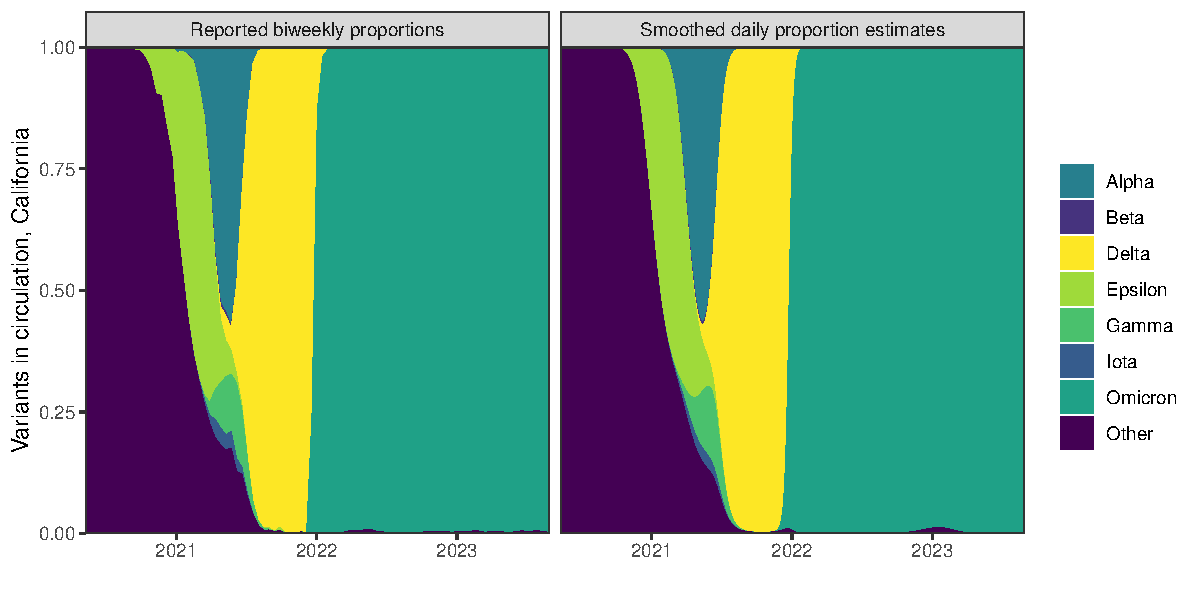
\includegraphics[width=\linewidth]{var-props-1.pdf}
        \caption{Left: Original biweekly proportions of the variants in circulation
        for California. Right: Daily proportions of the variants in circulation for
        California.}
        \label{fig:prop_figs}
    \end{figure}


    


\section{Constructing the delay from infection to test}
\label{sec:delay-sops}

The result of Step 1 (\Cref{sec:step1}) is $\widehat{x}_{\ell,t}$, case
estimates by positive specimen date for each state. To continue, pushing this
back to infection estimates, we need the variant-specific delays from infection
to positive specimen collection. As shown in \Cref{fig:chain_events_onset_report}, this delay can be broken into two separate pieces: (1) the
delay from infection to symptom onset, and (2) the delay from symptom onset to
positive specimen collection. The first requires different methods and is
specific to the variant causing the infection, while the second is estimable from the CDC line
list.

\section{Estimating the incubation period distributions} 
\label{sec:incubation}

To account for the incubation period, the time between infection and symptom
onset, we use estimates from the existing literature, modified slightly for
coherence with each other: we model each incubation as a gamma distribution with
different parameters. We focus on the following eight variants (shown in
\Cref{fig:prop_figs}), which saw significant circulation in one of the \US states
during our study period: Ancestral/Other, Alpha, Beta, Epsilon,
Iota, Gamma, Delta, and Omicron. Alpha, Beta, Delta, Gamma, and Omicron are all
variants of concern \citep{who2021tracking}, while we include the Epsilon
(California) and Iota (New York) variants because of large impact on those and
neighbouring states \citep{yang2022investigation, duerr2021dominance}.

The incubation period of the Ancestral variant has been modelled as a gamma
distribution \citep{tindale2020evidence}, so we simply use the reported shape
and scale parameters. For the Alpha, Beta, Gamma, Delta and Omicron variants,
the mean and standard deviation are reported \citep{tanaka2022shorter,
grant2022impact, ogata2022shorter}. Therefore, we use method of moments to match
the mean and variance to estimate the gamma parameters, using the moment
equations given in \Cref{sec:step1}. Then, we discretize each resulting density
shown in \Cref{fig:inc_gammas} to the support set, which is taken to be from 1
and 21 days. This range assumes that symptoms require at least 1 day to develop
\citep{phcan2021covid} and that an asymptomatic infection will resolve within
21 days \citep{zaki2021estimations,cortes2022sars}.

We were unable to locate incubation period estimates for the geo-specific
Epsilon and Iota variants, so we use the incubation period for Beta because
Epsilon, Iota, and Beta are all children from the same parent in the
phylogenetic tree of the Nextstrain Clades \citep{hodcroft2021covariants}. All
other circulating variants are grouped together with the Ancestral variant.
There was little available sequencing data prior to Alpha-emergence, but
unfortunately, later in the pandemic, it is impossible to separate Ancestral
from other rare variants, though these also saw minimal circulation after
the middle of 2021.

\begin{figure}[!tb]
\centering
    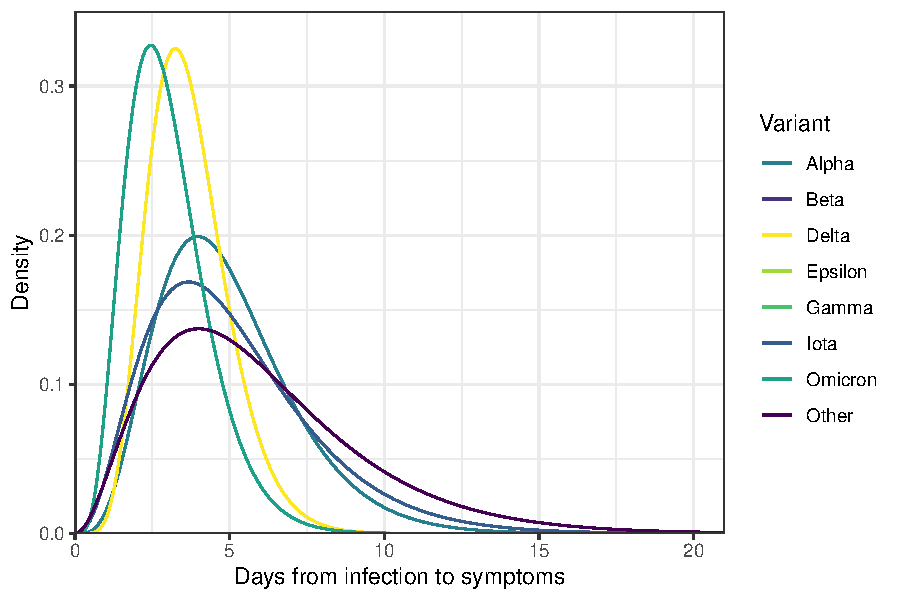
\includegraphics[width=0.6\linewidth]{inc-gammas-1.pdf}
    \caption{Gamma density for the incubation period of each of the eight
    variant categories. Note that the Ancestral variant uses reported shape and
    scale parameters \citep{tindale2020evidence}, while the remaining variants
    convert reported estimates for the mean and variance
    \citep{tanaka2022shorter,grant2022impact,ogata2022shorter} using the method
    of moments to produce the gamma parameters.}
    \label{fig:inc_gammas}
\end{figure}





\section{Estimating the delay distributions for symptom onset to positive specimen}
\label{sec:delay-sops}


Estimating the delay from symptom onset to positive specimen date follows a
similar procedure as described in \Cref{sec:step1} with a minor
adjustment. Here, we allow $k$ to range from $-3$ to $21$ (rather than $1$ to
$60$). These upper and lower bounds are based on the largest delay values for
the state-wide 0.05 and 0.95 quantiles. The median
delay is very short at approximately 2 days, and an asymptomatic individual may
test positive following a known exposure, before the onset of symptoms. We show
both types of delays for a sample of states over several dates in
\Cref{fig:delay-plots-samp}. Unlike the delay from positive specimen collection
to report, the delay from symptoms to positive specimen can conceivably be
negative. The most obvious reason for this would be if a person knew they had been
exposed to an infectious individual and so got tested prior to the development
of symptoms. Required regular testing for jobs in health care settings,
construction, or the film industry could also produce negative delays.


\begin{figure}[t!]
\centering
    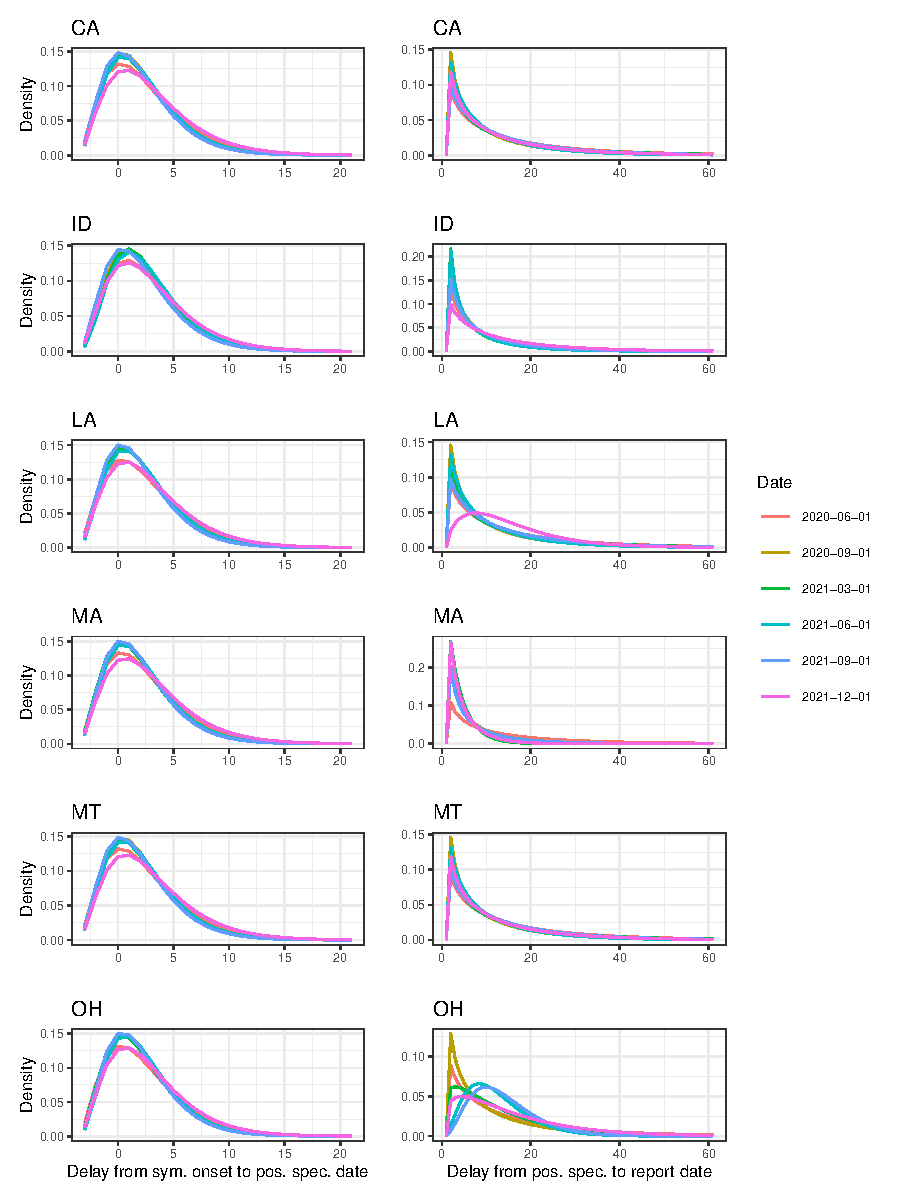
\includegraphics[width=.80\textwidth]{delay_plots.pdf} 
    \caption{Depictions of the estimated delay from symptom onset to
    positive specimen date (left) and from positive specimen date to report date
    (right) for a sample of six states over several dates.}
    \label{fig:delay-plots-samp}
\end{figure}

\section{Details on constructing the infection-to-test distributions}
\label{sec:details-conv}

Finally, to produce the delay from infection to positive specimen collection we
convolve the variant-specific incubation periods from \Cref{sec:incubation},
denoted by $\{i_{j}(k) : 0 < k \leq 21\}$ with the location-time-specific
symptom-to-positive-test distributions from \Cref{sec:delay-sops}, denoted by
$\{q_{\ell,t}(k) : -3\leq k \leq 21\}$. The convolution of these yields a
distribution $\{\tau_{j\ell,t}(k): -3 \leq k
\leq 42\}$. \Cref{fig:delay-plots-samp} shows the delays used for a sample of 6
states: symptom to positive specimen (left column) and positive specimen to report
(right column). The convolution distribution $\tau_{j\ell,t}$ requires
convolving the distribution in the left column with the variant-specific
incubation periods shown in \Cref{fig:inc_gammas}.





\section{Details about seroprevalence data}
\label{sec:sero-details}

We use two major contemporaneous surveys to estimate the proportion of the
population with evidence of previous infection in each state over time: the
2020--2021 Blood Donor Seroprevalence Survey and the Nationwide Commercial Lab
Seroprevalence Survey \citep{cdc2021blood, cdc2021comm}. In the former, the CDC
collaborated with 17 blood collection organizations in the largest nationwide
COVID-19 seroprevalence survey to date \citep{cdc2021blood}. The blood donation
samples were used to construct monthly seroprevalence estimates for nearly all
states from July 2020 to December 2021 \citep{jones2021estimated}. In the latter
survey, the CDC collaborated with two private commercial laboratories to test
blood samples from people that were in for routine or clinical management
(presumably unrelated to COVID-19 \citealp{bajema2021estimated}) for the
antibodies to the virus. The resulting dataset contains seroprevalence estimates
for a number of multi-week collection periods starting in July 2020 to February
2022. 

Both datasets are based on repeated, cross-sectional studies that estimate the
percentage of people who were previously infected with COVID-19 using the
percentage of people from a convenience sample who had antibodies against the
virus \citep{bajema2021estimated, cdc2020data, jones2021estimated}. Adjustments
were made in both for age and sex to account for the demographic differences
between the sampled and the target populations. However, both datasets are
incomplete and they differ in the number and the timing of the data points for
each state (\Cref{fig:sero-blood-comm-compar}). For example, in the
commercial dataset, the last estimate for North Dakota is in September 2020. In
the blood donor dataset, Arkansas does not have estimates available until
October 2020. 

\begin{figure}[!tb]
\centering
    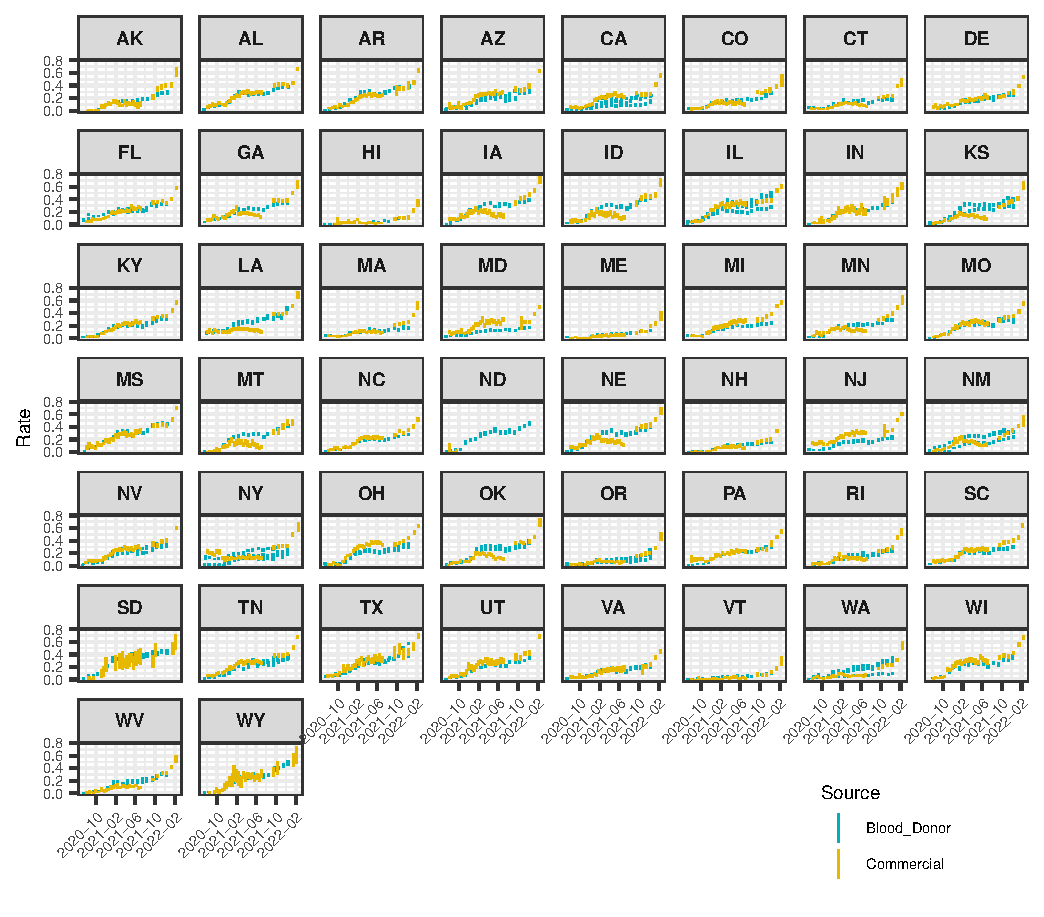
\includegraphics[width=.99\textwidth]{sero_blood_comm_compar.pdf}
    \caption{A comparison of the seroprevalence estimates from the Commercial
    Lab Seroprevalence Survey dataset (yellow) and the 2020--2021 Blood Donor 
    Seroprevalence Survey dataset (blue). Note that the maximum and the minimum
    of the line ranges are the provided 95\% confidence interval bounds to 
    give a rough indication of uncertainty.}
    \label{fig:sero-blood-comm-compar}
\end{figure}
    
A major difference in the structure of the two datasets is that the commercial
dataset always has the seroprevalence estimates at the level of the state, while
the blood donor dataset can either have estimates for the state or for multiple
separate regions within the state. For the commercial dataset, we use the
midpoint of the provided specimen collection date variable.  For the blood donor
dataset, we use the median donation date if the seroprevalence estimates are
designated to be for entire state. If they are instead for regions in the state,
since there is reliably one measurement per region per month, we aggregate the
measurements into one per month per state by using a weighted average (to
account for the given sample sizes of the regions). The median of the median
dates is taken to be the date for the weighted average. If there are multiple
measurements in a week from a seroprevalence source, then the average is used.


\section{State space representation of the antibody prevalence
model}\label{sec:ssapm} 
\begin{linenomath*}
\postdisplaypenalty=0
The antibody prevalence model described in \Cref{sec:report-ratio} can be expressed
as a linear Gaussian state space model \citep{durbin2012time}.
For $m = 1, \dots, M$, let $\alpha_m$ be a vector of
latent state processes at time $m$ and $y_m$ be a vector of
observations at time $m$. The form of the (general) linear Gaussian state space model is 
\begin{align}
y_m &= Z\alpha_m + \sigma^2_r\epsilon_m, \qquad \epsilon_m \sim N(0, H_m) \label{eq:ss1}\\
\alpha_{m+1} &= T_m\alpha_m + R\eta_m, \quad \eta_m \sim N(0, Q) \label{eq:ss2}
\end{align}
\end{linenomath*}
where $\alpha_1 \sim N(a_1, P_1)$ and 
$\epsilon_m$ and $\eta_m$ are mutually and serially independent.

% Kalman filtering gives the following one-step-ahead predictions of the states
% \begin{align*}
% a_{t+1} &= \E[\alpha_{t+1}\given y_t, \dots, y_1] 
% \end{align*} with covariance,
% \begin{align*}
% P_{t+1} &= \Var(\alpha_{t+1} \given y_t, \dots, y_1).
% \end{align*}
% Then, the Kalman smoother works backwards to the first time to give
% \begin{align}
% \hat{a}_t &= \E[\alpha_{t}\given y_n, \dots, y_1] \label{eq:hatat}\\
% V_t &= \Var(\alpha_{t}\given y_n, \dots, y_1). \label{eq:Vt}
% \end{align}
% The filtering and smoothing steps are based on recursions that are described in
% Appendix A of \citep{helske2017kfas} as we use the R package KFAS to estimate
% our model.

% For our situation, the Kalman filter and smoothing approach offers a number of
% advantages over the penalized regression approach. Perhaps most notably,
% the parameters are estimated all at once (so cross validating for model
% parameter tuning is not necessary). Another major benefit is that it can handle 
% unevenly spaced time series (refer to \citealp{durbin2012time} for further details).

To express the antibody prevalence model in state space form, we relate the
model in \Crefrange{eq:sero-measurements}{eq:report-ratio} to the components in
\Cref{eq:ss1,eq:ss2} as follows (omitting the location subscript for
simplicity):
\begin{linenomath*}
\begin{align}
    Z &= \begin{bmatrix} 1 & 0 & 0 & 0 \\ 0 & 1 & 0 & 0 \end{bmatrix} &
    H_m &= \begin{bmatrix}w^1_{m}\sigma^2_r & 0 \\ 0 & w^2_{m}\sigma^2_r \end{bmatrix} \\
    \alpha_m &= \begin{bmatrix}s_{m} \\ a_m \\ a_{m-1}\\ a_{m-2} \end{bmatrix} & 
    T_m &= \begin{bmatrix}(1 - \gamma) & \widehat{u}^\Sigma_{m} (1 - z_m) & 0 & 0\\ 
        0 & 3 & -3 & 1 \\ 0 & 1 & 0 & 0\\ 0 & 0 & 1 & 0 \end{bmatrix}  & 
    R &= \begin{bmatrix}1 & 0  \\ 0 & 1 \\ 0 & 0 \\ 0 & 0 \end{bmatrix}\\
    Q &= \begin{bmatrix} \sigma^2_\epsilon & 0  \\ 0 & \sigma^2_\eta \end{bmatrix} &
    a_1 &= \begin{bmatrix} \tilde{s}_{1}\\ \tilde{a}_1\\ \tilde{a}_1 \\ \tilde{a}_1 \end{bmatrix} & 
    P_{1} &= \begin{bmatrix} \sigma^2_{\tilde{s}_{1}} & 0 & 0 & 0 \\ 
    0 & \sigma^2_{\tilde{a}_1} & 0 & 0\\ 0 & 0 & \sigma^2_{\tilde{a}_1} & 0 \\ 
    0 & 0 & 0 & \sigma^2_{\tilde{a}_1} \end{bmatrix} 
\end{align}
\end{linenomath*}
where $\sigma^2_r$ is the variance of observations, $\sigma^2_\epsilon$ is the
variance of the seroprevalence estimates, $\sigma^2_\eta$ is the trend variance,
and $\widehat{u}^\Sigma_{m}$ denotes the new deconvolved cases between $m$ and
$m+1$. Because the inverse reporting ratios should be more variable than the
seroprevalence estimates, we enforce that the estimate of $\sigma^2_\eta$ is a
multiple of $\sigma^2_\epsilon$. 

Finally, $w^1_{m}$ and $w^2_{m}$ are the time-varying inverse variance weights
computed from the commercial and blood donor datasets, respectively. For each
source, we compute the weights for the observed seroprevalence estimates using
the formula for the standard error of a proportion. These weights are then
re-scaled to sum to the number of observed seroprevalence measurements for the
source. Finally, the ratio of the average observed weights from the two sources
is used to scale all weights relative the commercial source. This transformation
is done purely for computational purposes to make estimation of the unknown
parameters easier.

The prior distribution for $\alpha_1$ is estimated using both data-driven
constraints and externally sourced information. The initial value of the
seroprevalence component, $\tilde{s}_{1}$ is the average of the initial
seroprevalence measurements from each source rounded down to two decimal places.
The corresponding initial variance estimate, $\sigma^2_{\tilde{s}_{1}}$, is
taken to be the mean of the standard errors of the two seroprevalence estimates.
For the initial value of the trend component, we use the inverse of the
ascertainment ratio estimate for each state as of June 1, 2020 from Table 1 in  
\citep{unwin2020state}.

The initial $\sigma^2_r$ is taken to be the average of the estimated variances
from the observed seroprevalence measurements regressed linearly on time.
The initial value of the multiplier is set to be $100$ for all states. The
$\sigma^2_\epsilon$ and $\gamma$ values are estimated separately for each state,
then fixed to their averages on the log-scale.

Following maximum likelihood estimation of remaining parameters we use the
Kalman filter to obtain the smoothed point estimates and variances of the weekly
inverse reporting ratios. We use forward and backward extrapolation to extend
these estimates outside of the observed seroprevalence range
\citep{durbin2012time}, followed by linear interpolation to produce daily
values. We then multiply these by the
corresponding deconvolved case estimates before converting to per-capita values.
Annual estimates of the state
populations as of July 1 of 2020 are taken from the Dec.\
2022 press release from the \US Census Bureau \citep{uscensus2022annual}.


% The $50$, $80$, and $95\%$ confidence intervals are constructed by taking a
% Bayesian view of the antibody prevalence model (refer to \ref{sec:bayeswaning} 
% for the Bayesian specification of the model). 
% That is, for each time, $t$, we obtain an estimate of the
% posterior variance of $a_t$, apply the deconvolved case estimate as a constant
% multiplier, and then use resulting variance to build a normal confidence
% interval about the infection estimate. We additionally enforce that the lower
% bound must be at least the deconvolved case estimate for the time under consideration.


% \section{Bayesian specification of the antibody prevalence
% model}\label{sec:bayeswaning} 
% In brief, the antibody prevalence model where we let
% $\beta = \left \{  \gamma, a_1,\dots, a_t \right \}$ and $X$ be the design
% matrix, corresponds to a Bayesian model with prior 
% \begin{align*}
%     \beta \sim N \left( 0,  \frac{\sigma^2 }{ \lambda} \left( A^TD^TDA 
%     \right)^{-1}  \right)
% \end{align*} and likelihood 
% \begin{align*}
%     s|X,\beta \sim N \left( X\beta, \sigma^2W^{-1} \right),
% \end{align*} where $A$ is indicator matrix save for the first column of $0$s 
% (corresponding to $\gamma$), $D$ represents the discrete derivative matrix of 
% order $3$, and $W$ is the inverse variance weights matrix. Then, the posterior 
% on $a_t$ is normally distributed with mean 
% \begin{align*}
%     \left ( X^TWX + \lambda A^TD^TDA \right )^{-1}X^TWs
% \end{align*} 
% and variance 
% \begin{align*}
%     \sigma^2 (X^TWX + \lambda A^TD^TDA)^{-1}.
% \end{align*}


% \section{Scaling by population}



\section{Ablation analysis of infection-hospitalization correlations}
\label{sec:ablation}
In this ablation study, the lagged correlation is re-computed by
using the following infection estimates: 1. those from
the deconvolution procedure under the assumption that the infection onset is the
same as the positive specimen date (i.e., excluding the positive specimen to
infection onset data and deconvolution); 2. those from the deconvolution
procedure under the assumption that the infection onset is the same as the
symptom onset date (excluding the incubation period data); 3. those from the
deconvolution procedure when utilizing all incubation period and delay data (the
deconvolved case estimates); 4. those from applying the antibody prevalence
model to produce estimates for both the reported and the unreported cases (the
infection estimates).

The results of this study are shown in \Cref{fig:abl-lag-cor}. From
this, we can see that the deconvolved case and infection estimates from the
intermediate steps are all leading indicators of hospitalizations. However, the
degree that each such set of estimates lead hospitalizations depend on its
location in the sequence of deconvolution steps and how close the estimates are to infection
onset. For example, the deconvolved cases by positive specimen date tend to
precede hospitalizations by about $11$ days, while those for the subsequent step
indicate that the deconvolved cases by symptom onset tend to precede
hospitalizations by a longer time of $13$ days. Finally, after adding the
variant-specific incubation period data into the deconvolution and obtaining the
deconvolved case estimates, we can observe that the reported infections precede
hospitalizations by about $19$ days. 

\begin{figure}[H]
\centering
     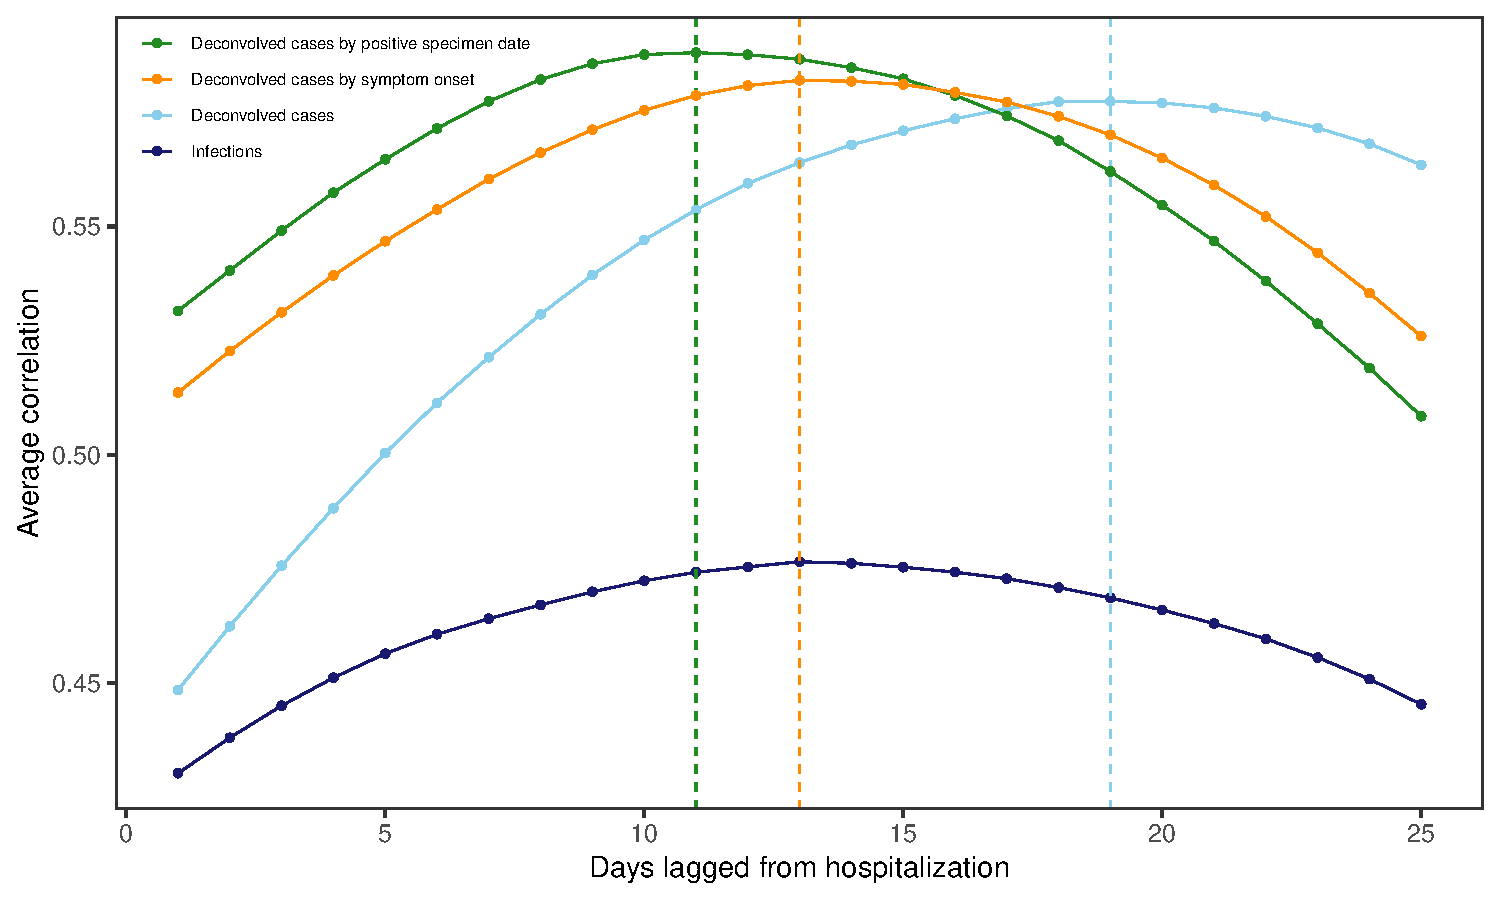
\includegraphics[width=.78\textwidth]{adj_unadj_pi_no_inc_hosp_lag_corr_F24.pdf} 
     \caption{Lagged Spearman's correlation between the infection and
     hospitalization rates per 100,000 averaged for each lag across \US states
     and days over June 1, 2020 to November 29, 2021, and taken over a rolling
     window of 61 days. The infection rates are based on the counts for the
     deconvolved case and infection estimates as well as the reported infections
     by symptom onset and when the report is symptom onset. Note that each such
     set of infection counts is subject to a center-aligned 7-day averaging to
     remove spurious day of the week effects. The dashed lines indicate the lags
     for which the highest average correlation is attained.}
     \label{fig:abl-lag-cor}
 \end{figure}
 